\documentclass{article}
\iffalse
This file is protected by Copyright. Please refer to the COPYRIGHT file
distributed with this source distribution.

This file is part of OpenCPI <http://www.opencpi.org>

OpenCPI is free software: you can redistribute it and/or modify it under the
terms of the GNU Lesser General Public License as published by the Free Software
Foundation, either version 3 of the License, or (at your option) any later
version.

OpenCPI is distributed in the hope that it will be useful, but WITHOUT ANY
WARRANTY; without even the implied warranty of MERCHANTABILITY or FITNESS FOR A
PARTICULAR PURPOSE. See the GNU Lesser General Public License for more details.

You should have received a copy of the GNU Lesser General Public License along
with this program. If not, see <http://www.gnu.org/licenses/>.
\fi

\author{} % Force author to be blank
%----------------------------------------------------------------------------------------
% Paper size, orientation and margins
%----------------------------------------------------------------------------------------
\usepackage{geometry}
\geometry{
	letterpaper,			% paper type
	portrait,				% text direction
	left=.75in,				% left margin
	top=.75in,				% top margin
	right=.75in,			% right margin
	bottom=.75in			% bottom margin
 }
%----------------------------------------------------------------------------------------
% Header/Footer
%----------------------------------------------------------------------------------------
\usepackage{fancyhdr} \pagestyle{fancy} % required for fancy headers
\renewcommand{\headrulewidth}{0.5pt}
\renewcommand{\footrulewidth}{0.5pt}
\rhead{\small{ANGRYVIPER Team}}
%----------------------------------------------------------------------------------------
% Appendix packages
%----------------------------------------------------------------------------------------
\usepackage[toc,page]{appendix}
%----------------------------------------------------------------------------------------
% Defined Commands & Renamed Commands
%----------------------------------------------------------------------------------------
\renewcommand{\contentsname}{Table of Contents}
\renewcommand{\listfigurename}{List of Figures}
\renewcommand{\listtablename}{List of Tables}
\newcommand{\todo}[1]{\textcolor{red}{TODO: #1}\PackageWarning{TODO:}{#1}} % To do notes
\newcommand{\code}[1]{\texttt{#1}} % For inline code snippet or command line
%----------------------------------------------------------------------------------------
% Various pacakges
%----------------------------------------------------------------------------------------
\usepackage{hyperref} % for linking urls and lists
\usepackage{graphicx} % for including pictures by file
\usepackage{listings} % for coding language styles
\usepackage{rotating} % for sideways table
\usepackage{pifont}   % for sideways table
\usepackage{pdflscape} % for landscape view
%----------------------------------------------------------------------------------------
% Table packages
%----------------------------------------------------------------------------------------
\usepackage{longtable} % for long possibly multi-page tables
\usepackage{tabularx} % c=center,l=left,r=right,X=fill
\usepackage{float}
\floatstyle{plaintop}
\usepackage[tableposition=top]{caption}
\newcolumntype{P}[1]{>{\centering\arraybackslash}p{#1}}
\newcolumntype{M}[1]{>{\centering\arraybackslash}m{#1}}
%----------------------------------------------------------------------------------------
% Block Diagram / FSM Drawings
%----------------------------------------------------------------------------------------
\usepackage{tikz}
\usetikzlibrary{shapes,arrows,fit,positioning}
\usetikzlibrary{automata} % used for the fsm
%----------------------------------------------------------------------------------------
% Colors Used
%----------------------------------------------------------------------------------------
\usepackage{colortbl}
\definecolor{blue}{rgb}{.7,.8,.9}
\definecolor{ceruleanblue}{rgb}{0.16, 0.32, 0.75}
\definecolor{drkgreen}{rgb}{0,0.6,0}
\definecolor{deepmagenta}{rgb}{0.8, 0.0, 0.8}
\definecolor{cyan}{rgb}{0.0,0.6,0.6}
\definecolor{maroon}{rgb}{0.5,0,0}
%----------------------------------------------------------------------------------------
% Update the docTitle and docVersion per document
%----------------------------------------------------------------------------------------
\def\docTitle{Component Data Sheet}
\def\docVersion{1.6}
%----------------------------------------------------------------------------------------
\date{Version \docVersion} % Force date to be blank and override date with version
\title{\docTitle}
\lhead{\small{\docTitle}}

\def\comp{fir\_real\_sse}
\edef\ecomp{fir_real_sse}
\def\Comp{FIR Real SSE}
\graphicspath{ {figures/} }

\begin{document}

\section*{Summary - \Comp}

\begin{tabular}{|c|M{13.5cm}|}
	\hline
	\rowcolor{blue}
	                  &                                                              \\
	\hline
	Name              & \comp                                                        \\
	\hline
	Worker Type       & Application                                                  \\
	\hline
	Version           & v\docVersion \\
	\hline
	Release Date      & 11/2019 \\
	\hline
	Component Library & ocpi.assets.dsp\_comps                                        \\
	\hline
	Workers           & \comp.hdl                                                    \\
	\hline
	Tested Platforms  & xsim, isim, centos 7 \\
	\hline
\end{tabular}


\begin{center}
	\textit{\textbf{Revision History}}
		\begin{table}[H]
		\label{table:revisions} % Add "[H]" to force placement of table
			\begin{tabularx}{\textwidth}{|c|X|l|}
			\hline
			\rowcolor{blue}
			\textbf{Revision} & \textbf{Description of Change} & \textbf{Date} \\
		    \hline
		    v1.4 & & 10/2018 \\
		    \hline
       	 	v1.5 &  & 4/2019 \\
		    \hline
		     v1.6 & Converted Worker to version 2 & 11/2019 \\
		    \hline
        		v1.7 & Addition of xilinx worker & 1/2020 \\
        		    & Table of Worker Configurations and Resource Utilization Table removed & 5/2020 \\
              \hline
			\end{tabularx}
		\end{table}
	\end{center}

\section*{Functionality}
\begin{flushleft}
	The FIR Real SSE (Systolic Symmetric Even) component inputs real signed samples and filters them based upon a programmable number of coefficient tap values. The underlying FIR Filter implementation makes use of a symmetric systolic structure to construct a filter with an even number of taps and symmetry about its midpoint.
\end{flushleft}

\section*{Worker Implementation Details}
\subsection*{\comp.hdl}
\subsubsection*{Filter taps}
\begin{flushleft}
	The \verb+NUM_TAPS_p+ parameter determines the length of the \verb+taps+ property.  Each 16-bit tap within the \verb+taps+ property is truncated by taking the \verb+COEFF_WIDTH_p+ number of least significant bits. Care should be taken to ensure that the \verb+COEFF_WIDTH_p+ parameter is $\le$ 16. The most significant bit of the truncated value is used as a sign bit. The truncated data is formatted as QN.0, where N is \verb+COEFF_WIDTH_p+-1. The truncated taps are effectively the first half of all coefficients used to perform convolution. The last half is equivalent to the reverse-indexed copy of the first half, allowing the coefficients to have symmetry about their midpoint. This symmetry of FIR coefficients results in group delay being constant across all frequencies.
\medskip
\end{flushleft}

\subsection*{Filter function}
\begin{flushleft}
	This implementation uses \verb+NUM_TAPS_p+ multipliers to process input data at the clock rate - i.e. this worker can handle a new input value every clock cycle. It is unnecessary to round the output data from this filter at the worker level because it is already being done within the macc\_systolic\_sym primitive.\medskip

	The FIR Real SSE worker utilizes the OCPI \textit{rstream\_protocol} for both input and output ports. The \textit{rstream\_protocol} defines an interface of 16-bit real signed samples. The \verb+DATA_WIDTH_p+ parameter may be used to reduce the FIR Real SSE hdl worker's internal data width to less than 16-bits.
\end{flushleft}
{\centering\captionsetup{type=figure}\includegraphics[scale=0.65]{fir_systolic_sym_even}\par\captionof{figure}{FIR Real SSE Block Diagram - 8-tap example}\label{fig:circuit}}

\subsection*{fir\_real\_sse\_for\_fskapp.rcc}
The RCC implementation for the fir\_real\_sse\_for\_fskapp worker in C++ is to function as a work-alike of the fir\_real\_sse.hdl in the FSK app. 
Since the RCC worker depends upon even symmetric taps architecture and liquid API used in this worker does not provide symmetric taps,
the required symmetric taps generation is done in this worker using C++ STD algorithm library. 
The fir\_real\_sse.hdl has a pipeline latency of \verb+NUM_TAPS_p+ + 4 clock cycles, and outputs \verb+NUM_TAPS_p+ + 3 zeros before the first filter output. This worker was written to function similar to fir\_real\_sse.hdl, and therefore has the same zeros-before-first-output behavior.

\subsection*{fir\_real\_sse\_for\_xilinx.hdl}
The implmentation based on Xilinx IP core is generated by Xilinx FIR Compiler. The default implementation uses 4 multipliers to process input data at one sample every 25 clock cycles. If a different rate is desired a new core can be recompiled. There is a startup latency of 36 clock cycles and the output is driven directly from the core's valid signal; therefore in simulations no delay will be observed. 

\section*{Theory}
\begin{flushleft}
	This filter will produce valid outputs one clock after each valid input, but care must be exercised when attempting to align outputs according to the filter's actual group delay and propagation delay.\medskip

	For a FIR filter with symmetric impulse response we are guaranteed to have linear phase response and thus constant group delay vs. frequency. In general, the group delay will be equal to (N-1)/2, where N is the number of filter taps.	The filter topology itself will add some propagation delay to the response. For this design the total delay from an impulse input to the beginning of the impulse response will be \verb+NUM_TAPS_p+ + 4 samples.
\end{flushleft}

\section*{Block Diagrams}
\subsection*{Top level}
\begin{center}
	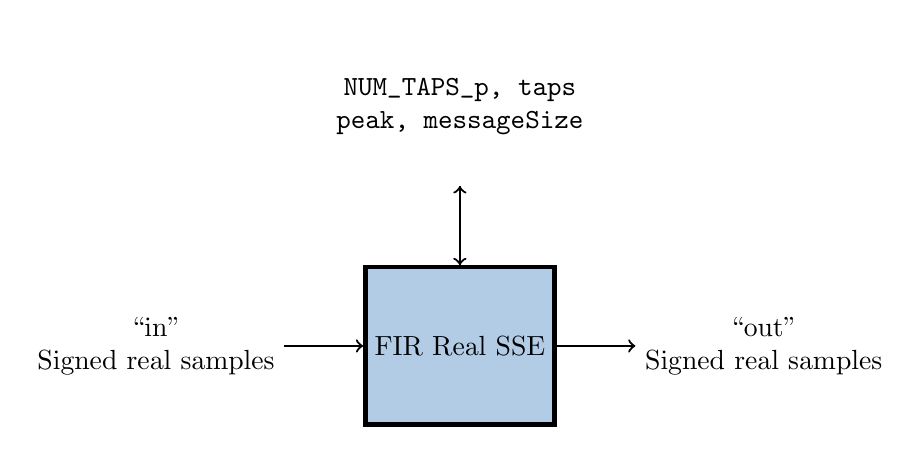
\begin{tikzpicture}[% List of styles applied to all, to override specify on a case-by-case
			every node/.style={
				align=center,  		% use this so that the "\\" for line break works
				minimum size=2cm	% creates space above and below text in rectangle
			},
			every edge/.style={draw,thick}
		]
		\node[rectangle,ultra thick,draw=black,fill=blue](R2){\Comp};
		\node[rectangle,draw=white,fill=white](R3)[left= of R2]{``in'' \\ Signed real samples};
		\node[rectangle,draw=white,fill=white](R4)[right= of R2]{``out'' \\ Signed real samples};
		\node[rectangle,draw=white,fill=white](R5)[above= of R2]{\verb+NUM_TAPS_p, taps+ \\ \verb+peak, messageSize+};
		\path[->]
		(R3)edge []	node [] {} (R2)
		(R2)edge []	node [] {} (R4)
		(R2)edge []	node [] {} (R5)
		(R5)edge []	node [] {} (R2)
		;
	\end{tikzpicture}
\end{center}


\newpage

\section*{Source Dependencies}
\subsection*{\comp.hdl}
\begin{itemize}
	\item assets/components/dsp\_comps/fir\_real\_sse.hdl/fir\_real\_sse.vhd
	\item assets/hdl/primitives/dsp\_prims/dsp\_prims\_pkg.vhd
	      \subitem assets/hdl/primitives/dsp\_prims/fir/src/fir\_systolic\_sym\_even.vhd
	      \subitem assets/hdl/primitives/dsp\_prims/fir/src/macc\_systolic\_sym.vhd
	\item assets/hdl/primitives/misc\_prims/misc\_prims\_pkg.vhd
	      \subitem assets/hdl/primitives/misc\_prims/round\_conv/src/round\_conv.vhd
	\item assets/hdl/primitives/util\_prims/util\_prims\_pkg.vhd
	      \subitem assets/hdl/primitives/util\_prims/pd/src/peakDetect.vhd
\end{itemize}
\subsection*{fir\_real\_sse\_for\_fskapp.rcc}
\begin{itemize}
	\item assets/components/dsp\_comps/fir\_real\_sse\_for\_fskapp.rcc/fir\_real\_sse\_for\_fskapp.cc
	      \subitem /opt/opencpi/prerequisites/liquid/include/liquid/liquid.h
	       
\end{itemize}
\subsection*{fir\_real\_sse\_for\_xilinx.hdl}
\begin{itemize}
	\item assets/components/dsp\_comps/fir\_real\_sse\_for\_xilinx.hdl/fir\_real\_sse\_for\_xilinx.vhd
		\subitem assets/components/dsp\_comps/fir\_real\_sse\_for\_xilinx.hdl/reload\_order\_rom.vhd
		\subitem assets/components/dsp\_comps/fir\_real\_sse\_for\_xilinx.hdl/gen/vivado\_ip/fir\_compiler\_0\_stub.vhd
          
\end{itemize}

\begin{landscape}
	\section*{Component Spec Properties}
	\begin{scriptsize}
		\begin{tabular}{|p{1.5cm}|p{1cm}|c|c|c|p{3cm}|c|p{7cm}|}
			\hline
			\rowcolor{blue}
			Name               & Type   & SequenceLength & ArrayDimensions   & Accessibility       & Valid Range                                                                      & Default & Usage                                                                        \\
			\hline
			\verb+NUM_TAPS_p+  & UChar  & -              & -                 & Parameter & 1-?                                                                              & 16      & Half the number of coefficients used by each           even symmetric filter \\
			\hline
			\verb+peak+        & Short  & -              & -                 & Volatile            & Standard                                                                         & 0       & Peak value of output (valid when PEAK\_MONITOR = true) \\
			\hline
			\verb+messageSize+ & UShort & -              & -                 & Writable & 8192                                                                             & 0       & Number of bytes in output message (Not implemented by Version 2)
			 \\
			\hline
			\verb+taps+        & Short  & -              & \verb+NUM_TAPS_p+ & Initial & -2\textsuperscript{COEFF\_WIDTH\_p-1} to +2\textsuperscript{COEFF\_WIDTH\_p-1}-1 & -       & Symmetric filter coefficient values                                          \\
			\hline
		\end{tabular}
	\end{scriptsize}

	\section*{Worker Properties}
	\subsection*{\comp.hdl}
	\begin{scriptsize}
		\begin{tabular}{|p{3cm}|p{2cm}|p{1cm}|c|c|c|c|c|p{5cm}|}
			\hline
			\rowcolor{blue}
			Type     & Name                 & Type  & SequenceLength & ArrayDimensions & Accessibility       & Valid Range & Default & Usage                                        \\
			\hline
			Property & \verb+DATA_WIDTH_p+  & UChar & -              & -               & Parameter & 1-16        & 16      & Data Width for internal processing \\
			\hline
			Property & \verb+COEFF_WIDTH_p+ & UChar & -              & -               & Parameter & 1-32        & 16      & Coefficient width in bits.                           \\
			\hline
			Property & \verb+PEAK_MONITOR+ & bool & -              & -               & Parameter &  -       & true      & Enable/Disable build-time inclusion of Peak Monitoring.                            \\
			\hline
		\end{tabular}
	\end{scriptsize}
 
 \subsection*{fir\_real\_sse\_for\_fskapp.rcc}
	\begin{scriptsize}
		\begin{tabular}{|p{3cm}|p{2cm}|p{1cm}|c|c|c|c|c|p{5cm}|}
			\hline
			\rowcolor{blue}
			Type     & Name                 & Type  & SequenceLength & ArrayDimensions & Accessibility       & Valid Range & Default & Usage                                        \\
			\hline
			Property & \verb+HDL_WORKER_DELAY+  & uchar & -              & -               & Parameter &    -   & 4      & The fir\_real\_sse.hdl worker has a 4 register delay.\\
			\hline
		\end{tabular}
	\end{scriptsize}

 \subsection*{fir\_real\_sse\_for\_xilinx.hdl}
	\begin{scriptsize}
		\begin{tabular}{|p{3cm}|p{2cm}|p{1cm}|c|c|c|c|c|p{5cm}|}
			\hline
			\rowcolor{blue}
			Type     & Name                 & Type  & SequenceLength & ArrayDimensions & Accessibility       & Valid Range & Default & Usage                                        \\
			\hline
			Property & \verb+PEAK_MONITOR+ & bool & -              & -               & Parameter &  -       & true      & Enable/Disable build-time inclusion of Peak Monitoring.                            \\
               \hline
			Property & \verb+COEFF_PADDING_p+  & uchar & -              & -               & Parameter &    -   & 2      & Numer of zero coefficients added to the beginning of filter.\\
			\hline
		\end{tabular}
	\end{scriptsize}
	
	\section*{Component Ports}
	\begin{scriptsize}
		\begin{tabular}{|M{2cm}|M{1.5cm}|M{4cm}|c|c|M{9cm}|}
			\hline
			\rowcolor{blue}
			Name & Producer & Protocol          & Optional & Advanced & Usage               \\
			\hline
			in   & false    & rstream\_protocol & false    & -        & Real signed samples \\
			\hline
			out  & true     & rstream\_protocol & false    & -        & Real signed samples \\
			\hline
		\end{tabular}
	\end{scriptsize}

	\section*{Worker Interfaces}
	\subsection*{\comp.hdl}
	\begin{scriptsize}
		\begin{tabular}{|M{2cm}|M{1.5cm}|c|c|M{12cm}|}
			\hline
			\rowcolor{blue}
			Type            & Name & DataWidth & Advanced                & Usage               \\
			\hline
			StreamInterface & in   & 16   & -     & Signed real samples \\
			\hline
			StreamInterface & out  & 16   & InsertEOM=1   & Signed real samples \\
			\hline
		\end{tabular}
	\end{scriptsize}
\end{landscape}

\section*{Control Timing and Signals}
\begin{flushleft}
	The FIR Real SSE HDL worker uses the clock from the Control Plane and standard Control Plane signals. The Raw Property interface is used to read/write coefficient values.
\end{flushleft}

\begin{landscape}
\section*{Worker Configuration Parameters}
\subsubsection*{\comp.hdl}
%\input{../../\ecomp.hdl/configurations.inc}
\section*{Performance and Resource Utilization}
\subsubsection*{\comp.hdl}
%\input{../../\ecomp.hdl/utilization.inc}
\end{landscape}
\section*{Test and Verification}

\begin{flushleft}
Two test cases are implemented to validate the FIR Real SSE component as dictated by parameter values for \verb+NUM_TAPS_p+: 16 and 128. In each case the python script \textit{gen\_lpf\_taps.py} is used to generate a taps file consisting of \verb+NUM_TAPS_p+ filter coefficients. Input data is generated by first creating a *.dat input file consisting of a single maximum signed value of +32767 followed by 2*(\verb+NUM_TAPS_p+-1) zero samples. The *.bin input file is the binary version of the *.dat ASCII file repeated 2*\verb+NUM_TAPS_p+ times.\medskip

The FIR Real SSE worker inputs real signed samples, filters the input as defined by the coefficient filter taps, and outputs real signed samples. Since the input consists of an impulse response - that is, a maximal `one' sample followed by all zeros equal to the length of the filter - the output is simply the coefficient values.\medskip

For verification, the output file is compared against the taps file, where a $\pm1$ difference is allowed in value while comparing the output against the filter coefficient values. Figures \ref{fig:out_time} and \ref{fig:out_freq} depict the filtered results of the impulse input for the case \verb+NUM_TAPS_p+=128.
\end{flushleft}

	\begin{figure}[ht]
		\centering
		\begin{minipage}{.5\textwidth}
			\centering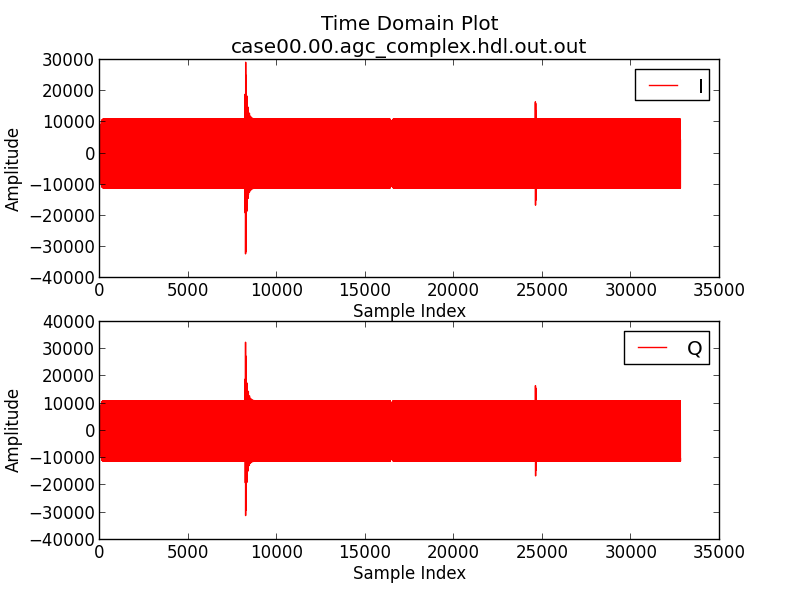
\includegraphics[width=1.0\linewidth]{output_time}
			\captionof{figure}{Time Domain Impulse Response}
			\label{fig:out_time}
		\end{minipage}%
		\begin{minipage}{.5\textwidth}
			\centering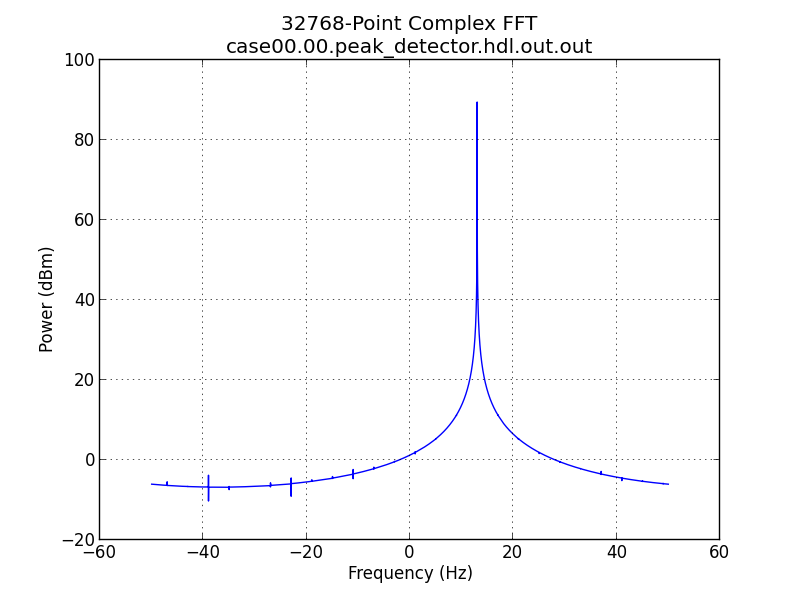
\includegraphics[width=1.0\linewidth]{output_freq}
			\captionof{figure}{Frequency Domain Impulse Response}
			\label{fig:out_freq}
		\end{minipage}
	\end{figure}
\end{document}
